\documentclass{article}

\usepackage[dutch]{babel}
\usepackage{epsfig}
\usepackage{verbatim}
\usepackage{moreverb}
\usepackage{float}
\usepackage{graphicx}
\usepackage{framed}
\usepackage{chngcntr}
\usepackage{enumitem}
\usepackage[font=bf]{caption}

\author{Peter van Dijk \& Elizabeth Schermerhorn}
\date{\today}
\title{Practicum 2 Synchronisatie bij vuurvliegjes}
\begin{document}
\maketitle
\newpage
\tableofcontents
\clearpage
\section{Inleiding}
In de natuur zijn er verschillende vormen van synchronisatie. Aangezien synchronisatie een belangrijk punt is in de werking tussen verschillende nodes in een netwerk is het van belang om een goed algoritme hiervoor te hebben. Een bekend voorbeeld uit de natuur zijn vuurvliegjes die met elkaar synchroniseren, wat zich uit in samen knipperen. Het algoritme dat vuurvliegjes gebruiken om synchroon te knipperen wordt ge\"{i}mplementeerd in een multi-hop netwerk. Door het algoritme te gebruiken moet het mogelijk zijn om nodes tegelijk te laten knipperen net zoals een groep vuurvliegjes. 
\section{Probleemstelling}
Het doel van dit onderzoek is het vinden van een algoritme om Arduino's te synchroniseren met behulp van radio's. Een aantal eisen waar dit algoritme aan moet voldoen zijn:
 \begin{itemize}
 \item Wanneer twee gesynchroniseerde netwerken worden samengevoegd dienen ze te synchroniseren.
 \item Wanneer een node uitvalt dient de synchronisatie nog te werken.
 \item Wanneer nodes toegevoegd worden aan het netwerk gaan deze met dezelfde frequentie knipperen als de andere nodes in het netwerk.
 \item Wanneer nodes uit synchronisatie raken moeten ze opnieuw synchroniseren. 
 \end{itemize}
Nu is vastgesteld aan welke eisen het algoritme moet voldoen kan er een hypothese opgesteld worden. Om ervoor te zorgen dat nieuwe nodes met dezelfde frequentie gaan knipperen als nodes die al langer in het netwerk verkeren zal er om de zoveel tijd opnieuw met alle nodes gesynchroniseerd moeten worden. Door dit in de implementatie toe te voegen zou dit ook moeten werken. Dit geldt ook voor de drie resterende bovengenoemde punten. 

\section{Gerelateerd werk}
Er zijn verschillende onderzoeken gedaan naar het onderwerp synchronisatie in een multi-hop netwerk. 
Een paar papers welke dit onderwerp aansnijden zijn: 
\begin{itemize}
	\item Clock synchronization for wireless sensor networks: a survey
	\item Wireless sensor network survey
	\item Academic Press Library in Signal Processing, Chapter 2 – Synchronization
\end{itemize}
De bovenstaande drie papers gaan over synchronisatie in draadloze netwerken. De eerste paper - Clock synchronization for wireless sensor networks: a survey - evalueert bestaande kloksynchronisatie-algoritmen gebaseerd op factoren zoals precisie, complexiteit, nauwkeurigheid en kosten \cite{survey}. De tweede paper, Wireless sensor network survey, geeft een overzicht van bestaande draadloze netwerk implementaties op verschillende niveaus \cite{survey2} en als laatste geeft het boek Academic Press Library in Signal Processing een kort overzicht van tijd synchronisatie in een netwerk \cite{academic}. \\
\\
In Sectie 3.3 van de paper "Clock synchronization for wireless sensor networks: a survey" wordt gesproken over de verschillende mogelijkheden bij de implementatie en hoe deze in hun werk gaan. 
Wanneer er een draadloos sensor netwerk ontwikkeld wordt zijn er een aantal factoren waar rekening mee gehouden moet worden. Hieronder staat een lijst weergegeven met de verschillende design-keuzes die gemaakt moeten worden.
\begin{itemize}
	\item Master-slave protocol versus peer-to-peer synchronisatie
	\item Interne synchronisatie versus externe synchronisatie
	\item Single-hop netwerk versus multihop netwerk
	\item probabilistische versus deterministische synchronisatie
\end{itemize}
In Sectie 3.3 van de paper "Clock synchronization for wireless sensor networks: a survey" staan nog meer keuzemogelijkheden, deze zijn niet van belang voor dit experiment en zijn voor het gemak weggelaten. 
In Appendix \ref{Terminologie} staat kort beschreven wat elke implementatiemogelijkheid inhoudt.\\
\\
Afhankelijk van de eisen die aan het netwerk gesteld worden moet er voor bepaalde onderdelen gekozen worden. Eisen aan het netwerk zouden kunnen zijn: Er is geen server beschikbaar, het moet zo min mogelijk energie verbruiken zodat de nodes lang meegaan of de nodes moeten over grotere afstand kunnen communiceren. Dit zijn slechts een aantal voorbeelden. \\
\\
In de tweede genoemde paper, Wireless sensor network survey, worden in sectie 6.2 meerdere synchronisatie-algoritmen uitgelegd. De volgende algoritmen worden beschreven:
\begin{itemize}
	\item Onzekerheid gedreven benadering
	\item Lucarelli's algoritme
	\item Vuurvlieg algoritme
	\item Tijd synchronisatie protocol voor sensor netwerken
	\item klok-opname gezamenlijke netwerk synchronisatie
	\item Tijd synchronisatie
	\item globale synchronisatie
	synchronisatie 
\end{itemize}
Het ge\"{i}mplementeerde algoritme dat in deze paper besproken wordt is gebaseerd op het vuurvliegalgoritme. Hoewel het ge\"{i}mplementeerde algoritme erop gebaseerd is, is het op sommige punten aangepast. 
Het vuurvliegalgoritme werkt als volgt: 
Elke node in het netwerk werkt als een oscillator met een vastgestelde tijd $T$. Elke node heeft een interne tijd $t$ die opgehoogd wordt totdat deze gelijk is aan $T$. Op tijd $T$ zal de node een signaal sturen en zijn interne tijd $t$ weer op $0$ zetten. Buren van deze node die dit signaal ontvangen zullen de tijd tussen $t$ en $T$ verkleinen. Dit wordt bepaald door middel van een functie en een kleine constante. Na verloop van tijd zullen de nodes gelijk hun signaal versturen dus gesynchroniseerd zijn. In Figuur \ref{fig: Firefly} is dit algoritme schematisch weergegeven. De bedoeling is dat alle nodes tegelijk een signaal gaan versturen na verloop van tijd.  
\begin{figure}[h]
\centering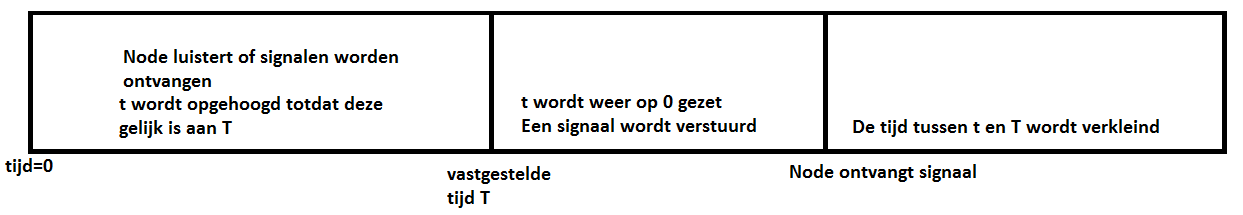
\includegraphics[scale=0.5]{Firefly}
\caption{Het vuurvliegalgoritme zoals beschreven in de paper}
\label{fig: Firefly}
\end{figure}
\begin{figure}[h]
\centering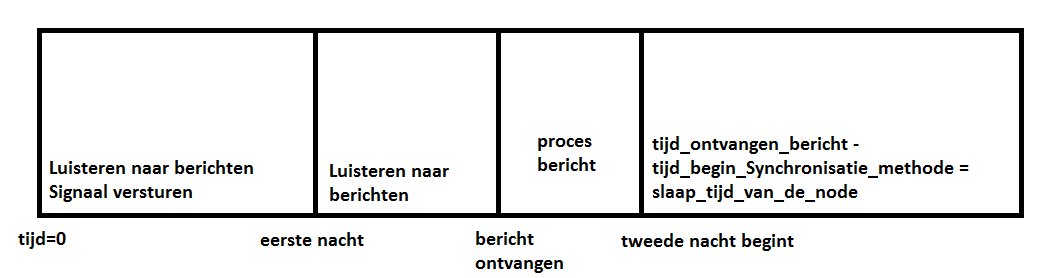
\includegraphics[scale=0.5]{Onze_implementatie}
\caption{Het ge\"{i}mplementeerde algoritme}
\label{fig: Onze_implementatie}
\end{figure}
Het grote verschil tussen bovenstaande implementatie en de experimentele implementatie van deze paper is dat de $t$ niet naar $0$ wordt gezet maar het verschil tussen het luisteren naar berichten en het uitlezen van de berichten wordt bijgehouden. Op basis van deze tijd wordt er voor een bepaalde tijd geslapen waardoor het tijdsverschil afneemt. Door dit fenomeen synchroniseren na verloop van tijd de nodes in het netwerk. 
\ref{fig: Onze_implementatie}

\section{Ontwerp synchronisatiealgoritme}
Het synchronisatie-algoritme is gebaseerd op een master-slave structuur. In Figuur \ref{fig: Schematisch} staat een schematische weergave van het netwerk zoals deze is gebruikt. Er zijn ID's meegegeven aan de nodes zodat er te zien is dat er \'{e}\'{e}n master is met \'{e}\'{e}n of meerdere slaves. 
\begin{figure}[h]
\centering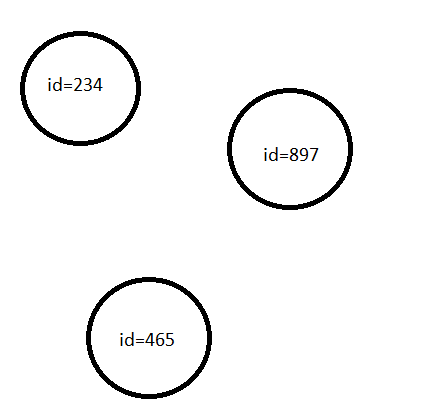
\includegraphics[scale=0.5]{testopstelling}
\caption{Schematische weergave van de testopstelling}
\label{fig: Schematisch}
\end{figure}
Iedere node in het network krijgt een willekeurig ID tussen de $0$ en de $1000$. De master van het netwerk wordt gekozen aan de hand van het hoogste ID. Er is gekozen voor deze structuur aangezien er gesynchroniseerd moet worden op een gekozen node. Het doel is om de nodes tegelijk te laten knipperen, om dit te laten werken moet de interne klok van de nodes gelijk lopen. In onze implementatie detecteert een node wanneer de master wakker is en zal zijn interne klok corrigeren naar dit moment. Binnen deze master-slave structuur is de implementatie verdeeld in twee alternerende delen.

!!!!!!!!!!!!!!!!!!!!!!!!!!!!!!!!!!!!!!!!!!!!!!!!!!!!!!!!!!!!!!!!!!!!!!!!!!!!!!!!!!!!!!
iets over bericht, iets over nacht
!!!!!!!!!!!!!!!!!!!!!!!!!!!!!!!!!!!!!!!!!!!!!!!!!!!!!!!!!!!!!!!!!!!!!!!!!!!!!!!!!!!!!!

In het eerste deel wordt een aantal maal achtereen alternerend de Arduino en Radio in slaapstand gezet en vervolgens een bericht verstuurd.

In het tweede deel wordt er gesynchroniseerd, eerst wordt er voor 
een nacht geluisterd of er berichten zijn ontvangen. Als er berichten zijn ontvangen worden deze verwerkt. Als laatste wordt er voor een nacht geslapen en als laatste wordt er een bericht gestuurd. 

Eerst zullen de gebruikte instellingen samen met het verstuurde signaal besproken worden. Daarna zullen de twee delen waaruit de implementatie bestaat toegelicht worden. 

\subsection{Gebruikte instellingen}
Omdat er gebruik wordt gemaakt van de RF24 radio om berichten te versturen zijn hier instellingen voor gebruikt. 
Instellingen gebruikt voor de RF24 radio:
\begin{itemize}
  \item hertransmissies: 0
  \item pakketgrootte: grote van bericht)
  \item geen automatische bevestiging bij ontvangen bericht
\end{itemize}
Om de pakketgrootte in te stellen wordt er gebruik gemaakt van de grootte van het bericht. Dit bericht is gedefini\"eerd in een  struct. Door dit struct te versturen kan er bij het ontvangen een bericht snel uitgelezen worden zonder delimiters te hoeven gebruiken. Deze struct bevat drie delen: ID van de zendernode, ID van de tot dan toe hoogst bekende node en het aantal verstuurde berichten. \\
\\
Er is gekozen om berichten een uniek nummer te geven per node, zodat verouderde berichten niet gebruikt worden om op te synchroniseren. Dit voorkomt dat nodes een ID van een uitgevallen node blijven versturen.
De hoogste ID is nodig om te beslissen of een bepaalde node de master node is en of daarnaar geluisterd moet worden. 
Als laatste is de ID van de Sender toegevoegd omdat dit de hoogste ID zou kunnen zijn in het netwerk. 
De instelling radio.setAutoAck(false); zorgt ervoor dat er geen acknowledgement wordt verstuurd op het moment dat er een bericht binnen komt. Dit is gedaan omdat er anders niet gesynchroniseerd kan worden, er zou op willekeurige momenten een bericht verstuurd worden. 
De laatste instelling, radio.setRetries(0,0);, houdt in dat wanneer het niet lukt op de vastgestelde tijd een bericht te sturen er geen hertransmissie plaats vindt. Anders zou een andere node die dit bericht ontvangt op het verkeerde moment gaan synchroniseren. 
Wat betreft de overige instellingen, is er gebruik gemaakt van de standaard instellingen van de arduino UNO en RF24.

\subsection{Het eerste deel, slapen en versturen}
Het eerste deel bestaat uit alternerend slapen en berichten versturen. 
\begin{verbatimtab}
int sendMax = 5;
int i = 0;
while(i<sendMax)
	sleepFor(1000)
	toggleLed();
	sendMessage();
	i++
\end{verbatimtab}
De bovenstaande pseudo code wordt vijf maal herhaald voordat er door wordt gegaan met het tweede deel.
Doordat er alleen berichten worden verstuurd over een lange periode is er een grote kans dat andere nodes de verzonden berichten ontvangen. Door voor vijf berichten te kiezen wordt deze kans alleen maar groter.

\subsection{Het tweede deel, synchroniseren}
Het tweede deel gaat over het synchroniseren van de nodes om ze tegelijk te laten knipperen. De synchronisatie gebeurt door de volgende acties:
\begin{verbatimtab}
listenFor(deltT)       //deltaT = Tijd tussen luisteren en uitlezen bericht
if(message_received){
	toggleLed();
} else {
	toggleLed(); 
	sendMessage();
}
sleepFor(1000 milliseconds);
toggleLed();
sendMessage();
\end{verbatimtab}
In bovenstaande code zal er eerst voor deltaT tijd geluisterd worden of er berichten worden ontvangen.
De tijd deltaT is de essentie van de synchronisatie en is de tijd die nodig is tussen het luisteren voor berichten en het daadwerkelijk verwerken van de ontvangen berichten. door zo lang te luisteren zullen alle nodes uiteindelijk synchroniseren. De berichten die van de master node komen en een hoger bericht nummer dan het laatst bekende zullen alleen verwerkt worden. 
Op het moment dat er een bericht is ontvangen zal alleen het LEDje getoggled worden. Anders zal er ook een nieuw bericht uitgezonden worden. Door hierna voor 1000 milliseconden te slapen blijft het LEDje of aan voor 1000 milliseconden of blijft uit voor 1000 milliseconden. Hierna zal opnieuw het LEDje getoggled worden en zal er weer een nieuw bericht verstuurd worden. Na deze synchronisatie periode zal er nu weer 5 maal deel \'{e}\'{e}n herhaald worden voordat deel twee weer herhaald wordt. 
\section{Testopstelling en resultaten van de test}
In deze paragraaf wordt het ge\"{i}mplementeerde algoritme onderzocht op hoe snale de synchronisatie plaatsvind bij verschillende afstanden. De hypothese is dat naarmate de afstand groter wordt de tijd om te synchroniseren toenaamt. Er is meer tijd nodig om de berichten te versturen dus zal het langer duren voor het synchroon gaat. De schematische opstelling hiervan is te zien in Tabel \ref{tab: testresultaten} en de re\"{e}le opstelling zoals deze was is te zien in Figuur \ref{fig: Nodes_tijdens_testen}. 
\begin{figure}[h]
\centering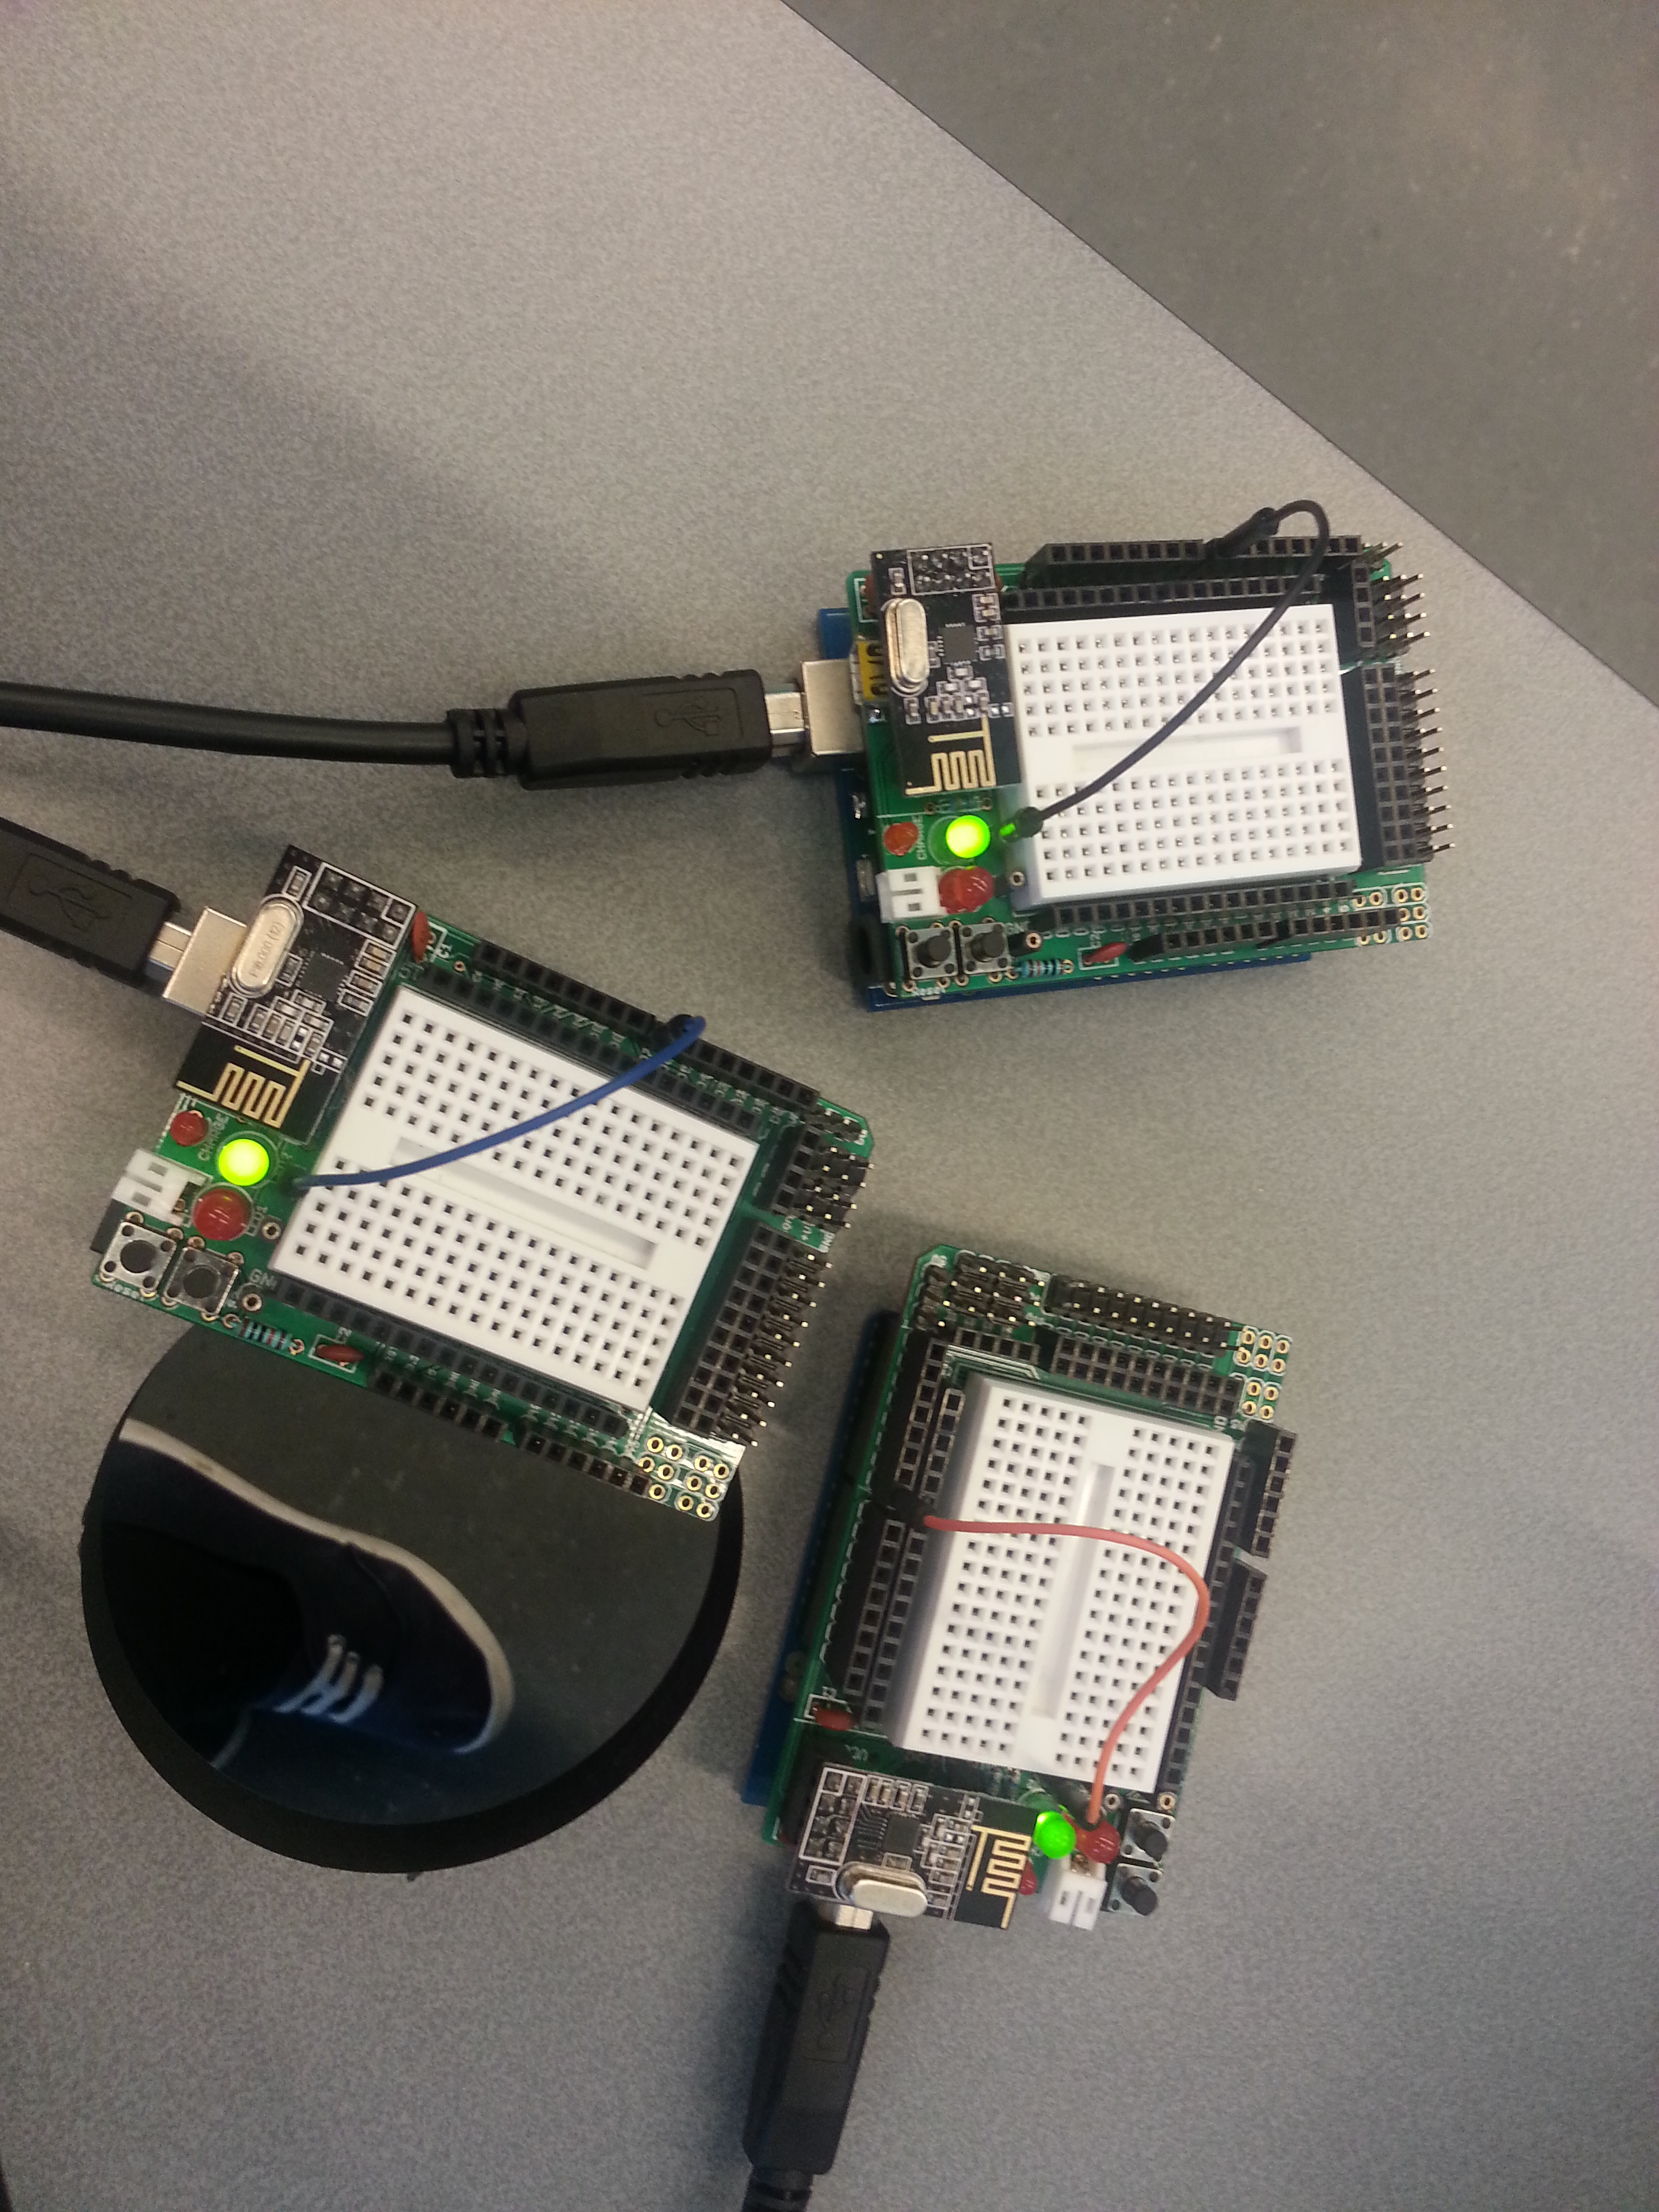
\includegraphics[scale=0.09, angle=90]{Nodes_tijdens_testen}
\caption{Testopstelling}
\label{fig: Nodes_tijdens_testen}
\end{figure}

    
\begin{table}[h]
	\centering\caption{Testresultaten}
	\label{tab: testresultaten}
    \begin{tabular}{| l | l | l | l |  l |}\hline
    \textbf{afstand } & \textbf{10 cm } & \textbf{25 cm} & \textbf{50 cm} & \textbf{100 cm} \\ \hline\hline
   1. & 4,33 seconden & 11,50 seconden& 7,40 seconden& 6,72 seconden\\ \hline
    2. & 4,72 seconden & 5,58 seconden& 17,46 seconden& 6,18 seconden\\ \hline
    3. & 4,07 seconden & 9,0 seconden& 8,84 seconden& 6,40 seconden\\ \hline
    4. & 3,82 seconden & 9,85 seconden& 12,54 seconden& 5,71 seconden\\ \hline
    5. & 7,92 seconden & 4,20 seconden& 8,87 seconden& 4,93 seconden\\ \hline \hline
   gemiddelde & 4.972 seconden & 8.026 seconden& 11.22 seconden& 5.988 seconden\\\hline
    \end{tabular}
\end{table}
In Tabel \ref{tab: testresultaten} is te zien hoe de afstand van de nodes zich verhoudt tot de tijd die het neemt om te synchroniseren. Wat opmerkelijk is aan deze tabel is dat met een afstand van 50 centimeter de synchronisatie tijd soms meer dan twee keer zo lang neemt als wanneer er op een afstand van 100 centimeter wordt gesynchroniseerd. Twee mogelijke verklaringen voor dit fenomeen zijn:
\begin{itemize}
	\item Door interferentie met wi-fi is er op bepaalde momenten soms meer of minder bereik van de radio's.
	\item door de gebruikte golflengtes van de radio kan het zijn dat er dode punten ontstaan zoals bij een satelliet. Er zijn bepaalde afstanden waar dit voor gebeurt en dit zou ook kunnen bij bijvoorbeeld 50 centimeter afstand. 
\end{itemize}
\section{Conclusie en aanbevelingen}
De probleemstelling die gesteld werd is: \textit{"het synchroniseren van nodes in een multihop netwerk met als doel ze tegelijk te laten knipperen."}. Na het testen van de implementatie kan er geconcludeerd worden dat het experiment geslaagd is en dus de hypothese waar is. In Tabel \ref{tab: Gestelde eisen} staan de eisen waar de implementatie aan voldoet. In het hoofdstuk :\textit{Ontwerp synchronisatie-algoritme} en in \textit{Testopstellingen en resultaten} staan de implementatie en de testresultaten. 
\begin{table}[h]
	\centering\caption{Gestelde eisen aan het netwerk}
	\label{tab: Gestelde eisen}
	\begin{tabular}{|l|p{10cm}|}\hline
	\textbf{nummer} & \textbf{eis} \\ \hline
	1. & Wanneer twee gesynchroniseerde netwerken worden samengevoegd 
	dienen ze te synchroniseren. \\ \hline
	2. & Wanneer een node uitvalt dient de synchronisatie 
	nog te werken. \\ \hline
	3. & Wanneer nodes toegevoegd worden aan het netwerk gaan deze met dezelfde
	 frequentie knipperen als de andere nodes in het netwerk.\\ \hline
	4. & Wanneer nodes uit sync raken moeten ze opnieuw synchroniseren. \\ \hline
	\end{tabular}
\end{table}
\newline
Hoewel de code werkt en de tests zijn gelukt staat de implementatie open voor verbetering. Tijdens dit onderzoek was er slechts de beschikbaarheid over drie nodes. In de subsectie aanbevelingen worden verder testmethoden en uitbreidingen voorgesteld. 
\subsection{Aanbevelingen}
Tijdens dit onderzoek was er slechts de beschikbaarheid over drie nodes. In een vervolgonderzoek kan er meer uitgebreid getest worden of het ook werkt met veel meer nodes. Vragen die hierbij gesteld kunnen worden zijn:
\begin{itemize}
	\item Is er een maximum aan het aantal nodes in het netwerk waarop er nog gesynchroniseerd kan worden? Aangezien er gebruik wordt gemaakt van een random getal tussen 0 en 1000 is het van belang om te weten wanneer er vaak dubbele getallen voorkomen. 
	\item veranderd de synchronisatie tijd die nodig is om te synchroniseren naarmate er meer nodes in het netwerk aanwezig zijn?
	\item De mogelijkheden onderzoeken om in plaats van een gedecentraliseerd netwerk te ontwikkelen een gecentraliseerd netwerk te synchroniseren. Gebruik makende van de code en hier enkele aanpassingen aan te maken. 
\end{itemize}
\newpage
%\section{References}
%\nocite{*} % Even non-cited BibTeX-Entries will be shown.
\bibliographystyle{abbrv}
\bibliography{literature}



\clearpage
\appendix
\counterwithin{figure}{section}
\section{Code Sender}
\verbatiminput{./code/node.ino}
\newpage

\section{Terminologie}

\label{Terminologie}
\begin{table}[H]
	\centering
	\caption{Toelichting op de implementatie mogelijkheden}
	\label{tab: implmentatie_mogelijkheden}
    \begin{tabular}{ | l | p{5cm} |}\hline
    
    \textbf{Onderdeel} & \textbf{Uitleg} \\ \hline\hline
    Master-slave protocol & Er is een master node in het netwerk waar alle andere nodes naar luisteren, deze bepaald de synchronisatie \\ \hline
    peer-to-peer protocol &  Elke node in het netwerk heeft contact met elke andere node. Dit elimineert het risico dat wanneer een master node wegvalt het netwerk niet meer synchroniseert.\\ \hline
    Interne synchronisatie & De re\"{e}le tijd is niet beschikbaar. Het doel is het verschil in tijd tussen de lokale klok en het uitlezen van de sensor zo klein mogelijk te maken.\\
    \hline
    externe synchronisatie & Hier is de tijd wel beschikbaar zoals UTC. Er is een atomische klok die de ware tijd heeft.\\
    \hline
    single hop netwerk & Elke node in het netwerk heeft contact met elke andere node in het netwerk\\
    \hline
    multi hop netwerk & Niet elke node in het netwerk heeft contact met een andere node in het netwerk. \\
    \hline
    probabilistische synchronisatie & Geeft een probabilistische garantie van de maximum offset van de klok. \\
    \hline
    deterministische synchronisatie & Deze algoritme garanderen een bepaalde maximum offset van de klok. \\
    \hline
    \end{tabular}
\end{table}

\end{document}
